\section{Застосування моделі лінійної парковки на практиці}

На перший погляд, суттєвим недоліком одновимірної моделі парковки є незастосовність до тих парковок, що зустрічаються у реальному житті. Насправді, це не так.

Майже кожна сучасна парковка складається з одного або кількох нахилених рядів, обмежених розміткою або огорожею. Але кожний такий ряд нескладно трансформувати у модель одновимірної парковки. Наприклад, на \imref{fig:model_application} зображено, як можна парковку, що складається з двох рядів, представити у вигляді суперпозиції двох моделей одновимірної парковки. Після цього можна застосовувати отримані результати для кожного ряду окремо.

\begin{figure}[bh]
	\begin{subfigure}[b]{0.49\textwidth}    
		\centering
		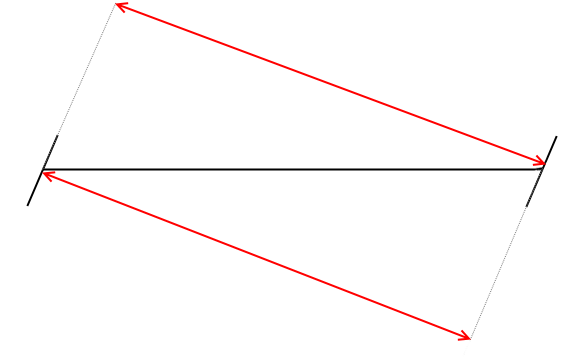
\includegraphics[width=1\linewidth]{chapter_Application/img/parking_real}
		\caption{}
	\end{subfigure}
	\begin{subfigure}[b]{0.49\textwidth}    
		\centering
		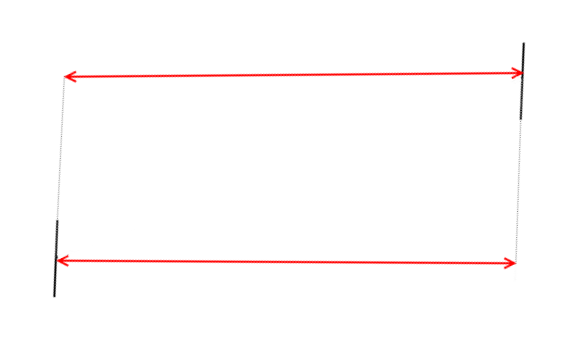
\includegraphics[width=1\linewidth]{chapter_Application/img/parking_real_transformed}
		\caption{}
	\end{subfigure}
	\caption{Схематичне зображення ряду з реальної парковки (а) та представлення у вигляді двох лінійних парковок (б)}
	\label{fig:model_application}
\end{figure}
